% "{'chapitre':'slci_laplace','classe':('PSI'),'type':('td','colle'),'titre':'Tour en fosse utilisé pour le reprofilage des roues ferroviaires', 'source':'Concours Centrale Supelec - PSI 2018','comp':['SLCI-09','SLCI-11',],'corrige':True}"

\setchapterimage{fig_00}
\renewcommand{\titrechapitre}{Tour en fosse utilisé pour le reprofilage des roues ferroviaires -- Asservissement du porte-outil}
\renewcommand{\leftmark}{\titrechapitre}
\renewcommand{\rightmark}{\titrechapitre}

\chapter*{\ifcolle Colle \arabic{cptColle}  \else TD \arabic{cptTD} \fi \\ 
\titrechapitre -- \ifprof Corrigé \else Sujet \fi}

\addcontentsline{toc}{section}{\ifcolle Colle \arabic{cptColle}  \else TD \arabic{cptTD} \fi  : \titrechapitre  -- \ifprof Corrigé \else Sujet \fi}

\iflivret \ifcolle \stepcounter{cptColle}  \else \stepcounter{cptTD} \fi   \else
\ifprof  \ifcolle \stepcounter{cptColle}  \else \stepcounter{cptTD} \fi \else \fi
\fi
\setcounter{question}{0}

\marginnote{Concours Centrale Supelec -- PSI 2018.}
%\marginnote{\UPSTIcompetence[2]{B2-07}
\marginnote{\xpComp{SLCI}{09}\xpComp{SLCI}{11}}
%\UPSTIcompetence[2]{C2-02}}
\begin{marginfigure}
\centering
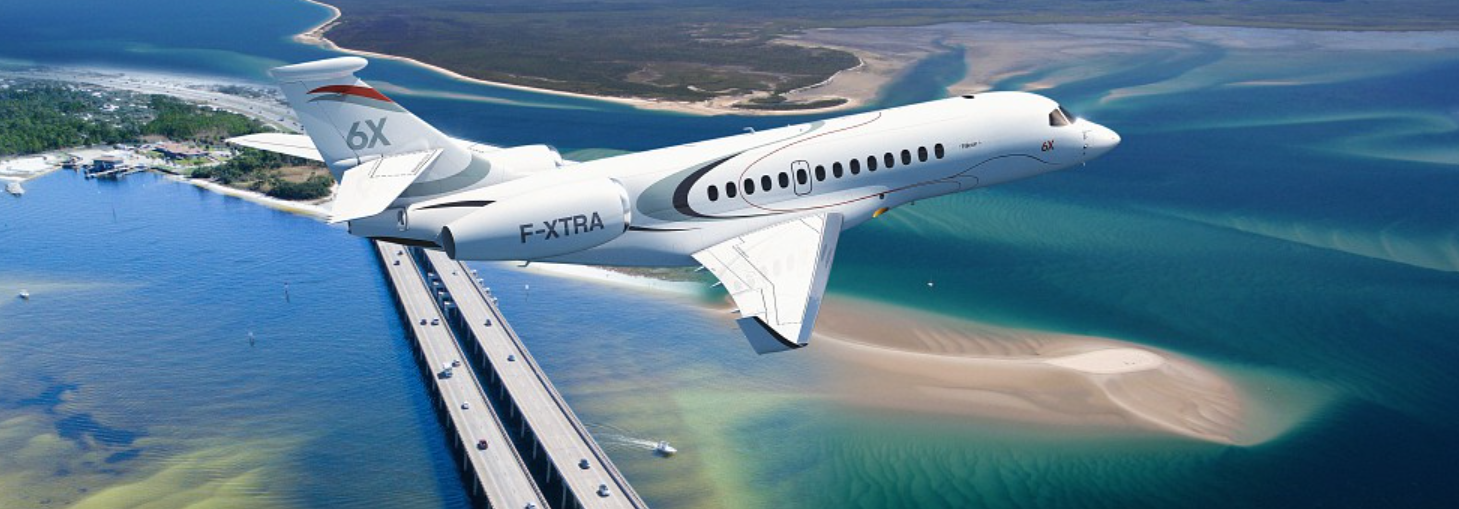
\includegraphics[width=.9\linewidth]{fig_00}
\end{marginfigure}



\subsection*{Modélisation du mouvement pour la commande}
\ifprof
\else
\begin{obj}
Modéliser le comportement dynamique de l’outil et du porte-outil, puis étudier une commande en
position $z_1(t)$ comprenant un correcteur proportionnel.
\end{obj}

Le système composé de l’outil et du porte-outil est modélisé sur la \autoref{fig_10}. Le porte-outil, de masse $m_1 = \SI{5522}{kg}$,
est considéré indéformable et en liaison glissière de direction $\vect{z_0}$ avec le bâti. Une chaîne de motorisation électrique
permet de déplacer le porte-outil et une structure de commande associée permet d’asservir la position
$z_1(t)$ par rapport à une position de référence. La chaîne de motorisation exerce une force motrice $\vect{f}_m(t) =f_m(t)\vect{z_0}$
sur le porte-outil.

La cahier des charges est donné sur la figure suivante.

\begin{figure}[H]
\centering
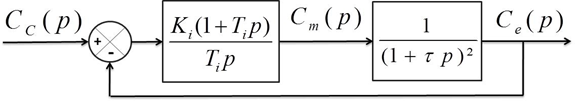
\includegraphics[width=.8\linewidth]{fig_08}
\caption{Diagramme des exigences de la chaîne d'asservissement \label{fig_08}}
\end{figure}


\begin{marginfigure}[-3cm]
\centering
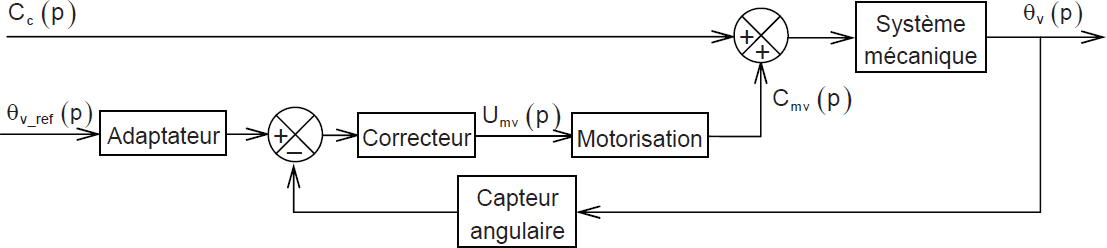
\includegraphics[width=\linewidth]{fig_10}
\caption{Modèle de déformation de l'outil avec le porte-outil piloté \label{fig_10}}
\end{marginfigure}

Les positions du porte-outil et du point $C$  par rapport à leur position de référence sont respectivement paramétrées
par $z_1(t)\vect{z_0}$ et $z_2(t)\vect{z_0}$, avec $z_1(t)\vect{z_0}$ et $z_2(t)\vect{z_0}$ des grandeurs algébriques (\autoref{fig_10}). Les conditions initiales
sont toujours supposées nulles.


Le théorème de la résultante dynamique appliqué au porte-outil puis à l’outil permet d’obtenir les deux relations
suivantes :
$$
\begin{array}{l}
m_1\ddot{z}_1(t)+\lambda\dot{z}_1(t)+Kz_1(t) = \lambda\dot{z}_2(t)+Kz_2(t)+f_m(t) \\
m_2\ddot{z}_2(t)+\lambda\dot{z}_2(t)+Kz_2(t) = \lambda\dot{z}_1(t)+Kz_1(t)+f_c(t) \\
\end{array} $$
Le modèle correspondant est représenté par le schéma bloc de la  \autoref{fig_11}.

\begin{marginfigure}
\centering
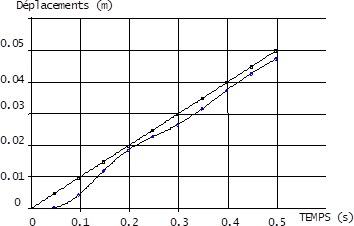
\includegraphics[width=\linewidth]{fig_11}
\caption{Modèle de l'outil et du porte-outil \label{fig_11}}
\end{marginfigure}

\fi

\question{Exprimer les fonctions $H_1(p)$, $H_2(p)$, $H_3(p)$ et $H_4(p)$ en fonction de $K$, $\lambda$, $m_1$ et $m_2$.}
\ifprof
\begin{corrige}
D'après le schéma-blocs $Z_1(p)=H_2(p)\left(F_m(p)+H_1(p)Z_2(p)\right)$. 
D'après la première équation différentielle, on a : $m_1p^2 Z_1(p) + \lambda pZ_1(p)+KZ_1(p)=\lambda pZ_2(p)+KZ_2(p)+F_m(p)\Leftrightarrow 
Z_1(p)\left(m_1p^2  + \lambda p+K \right)=Z_2(p)\left(\lambda p+K\right)+F_m(p)
\Leftrightarrow 
Z_1(p)= \dfrac{Z_2(p)\left(\lambda p+K\right)+F_m(p)}{m_1p^2  + \lambda p+K}$.
On a donc par identification $H_2(p)=\dfrac{1}{m_1p^2  + \lambda p+K}$ et $H_1(p)=\lambda p+K$.

D'après le schéma-blocs $Z_2(p)=H_4(p)\left(F_c(p)+H_3(p)Z_1(p)\right)$. D'après la seconde équation différentielle,  $m_2p^2 Z_2(p) + \lambda pZ_2(p)+KZ_2(p)=\lambda pZ_1(p)+KZ_1(p)+F_C(p)\Leftrightarrow Z_2(p)\left( m_2p^2  + \lambda p+K \right)=Z_1(p)\left(\lambda p+K\right)+F_C(p)\Leftrightarrow Z_2(p)=\dfrac{Z_1(p)\left(\lambda p+K\right)+F_C(p)}{ m_2p^2  + \lambda p+K}$.
On a donc par identification $H_4(p)=\dfrac{1}{m_2p^2  + \lambda p+K}$ et $H_3(p)=\lambda p+K$.

Au final, 
$$
H_1(p)=\lambda p+K \quad 
H_2(p)=\dfrac{1}{m_1p^2  + \lambda p+K} \quad 
H_3(p)=\lambda p+K  \quad 
H_4(p)=\dfrac{1}{m_2p^2  + \lambda p+K} 
$$
\end{corrige}
\else
\fi

\ifprof

\else

\begin{marginfigure}
\centering
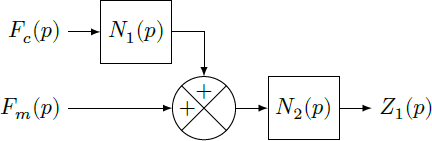
\includegraphics[width=\linewidth]{fig_12}
\caption{Modèle équivalent \label{fig_12}}
\end{marginfigure}

Le modèle de la  \autoref{fig_11} est réduit au modèle équivalent de la figure \autoref{fig_12}.

\fi

\question{Exprimer $N_1(p)$ et $N_2(p)$ en fonction de $H_1(p)$, $H_2(p)$, $H_3(p)$ et $H_4(p)$.}
\ifprof
\begin{corrige}
En utilisant le premier modèle, on avait :
$
\left\{\begin{array}{l}
Z_1(p)=H_2(p)\left(F_m(p)+H_1(p)Z_2(p)\right) \\
Z_2(p)=H_4(p)\left(F_c(p)+H_3(p)Z_1(p)\right)
\end{array}
\right.
$. 

Ainsi, $Z_1(p)=H_2(p)\left(F_m(p)+H_1(p)\left( H_4(p)\left(F_c(p)+H_3(p)Z_1(p)\right)\right)\right) $

$=H_2(p)F_m(p)+H_1(p)H_2(p) H_4(p)F_c(p)+H_1(p)H_2(p) H_3(p)H_4(p)Z_1(p) $

$\Leftrightarrow Z_1(p)\left( 1-H_1(p)H_2(p) H_3(p)H_4(p)\right)=H_2(p)\left(F_m(p)+H_1(p)H_4(p)F_c(p)\right) $. 

En utilisant le schéma-blocs, $Z_1(p)=\left(F_c(p)N_1(p)+F_m(p)\right)N_2(p)$. 
Par identification, on obtient $N_1(p)=H_1(p)H_4(p)$ et $N_2(p)=\dfrac{H_2(p)}{1-H_1(p)H_2(p) H_3(p)H_4(p)}$.

\end{corrige}
\else
\fi

\question{Montrer que $N_2(p)$ peut s’écrire sous la forme $N_2(p) = A\dfrac{p^2+2\xi_1\omega_1 p + \omega_1^2}{p^2\left( p^2+2\xi_2\omega_2p + \omega_2^2\right)}$. Exprimer $\xi_1$, $\xi_2$, $\omega_1$, $\omega_2$ et $A$ en fonction de $m_1$n $m_2$, $\lambda$ et $K$.}
\ifprof
\begin{corrige}
$N_2(p)=\dfrac{H_2(p)}{1-H_1(p)H_2(p) H_3(p)H_4(p)}$ 
$= \dfrac{\dfrac{1}{m_1p^2  + \lambda p+K}}{1-\left(\lambda p+K\right)\dfrac{1}{m_1p^2  + \lambda p+K} \left(\lambda p+K\right)\dfrac{1}{m_2p^2  + \lambda p+K}}$

$= \dfrac{1}{\left(m_1p^2  + \lambda p+K\right)- \dfrac{\left(\lambda p+K\right)^2}{m_2p^2  + \lambda p+K}}$
$= \dfrac{m_2p^2  + \lambda p+K}{\left(m_1p^2  + \lambda p+K\right)\left(m_2p^2  + \lambda p+K\right)- \left(\lambda p+K\right)^2}$

$= \dfrac{m_2p^2  + \lambda p+K}{
m_2m_1p^4  + \lambda m_1p^3+Km_1p^2+\lambda m_2p^3  + \lambda^2 p^2 +\lambda pK+Km_2p^2  + K\lambda p+K^2 - \lambda^2 p^2 -K^2 - 2\lambda p K}$

$= \dfrac{m_2p^2  + \lambda p+K}{
m_2m_1p^4  + \lambda m_1p^3+Km_1p^2+\lambda m_2p^3   +Km_2p^2 }$
$= \dfrac{m_2p^2  + \lambda p+K}{
p^2\left( m_1m_2p^2  + \left(m_1+ m_2\right) \lambda p  +K\left(m_1+m_2\right)\right) }$

$= \dfrac{m_2\left(p^2  + \dfrac{\lambda}{m_2}p+\dfrac{K}{m_2}\right)}{
p^2 m_1m_2 \left(p^2  + \dfrac{m_1+ m_2}{m_1m_2} \lambda p  +K\dfrac{m_1+m_2}{m_1m_2}\right) }$.

Par identification, on a : $A=\dfrac{1}{m_1}$, $\omega_1^2=\dfrac{K}{m_2}$, $2\xi_1\omega_1=\dfrac{\lambda}{m_2}$ et $\xi_1 = \dfrac{\lambda}{2 \omega_1 m_2}=\dfrac{\lambda}{2 \sqrt{Km_2}  } = $, $\omega_2^2=K\dfrac{m_1+m_2}{m_1m_2}$, $2\xi_2\omega_2=\lambda\dfrac{m_1+ m_2}{m_1m_2}$ et $\xi_2 = \dfrac{\lambda}{2}\sqrt{\dfrac{m_1+m_2}{m_1m_2 K}}$. 

On a donc $\xi_1=\dfrac{\lambda}{2  \sqrt{m_2K}}$ et 
$\xi_2=\lambda\dfrac{\sqrt{m_1+ m_2}}{2\sqrt{Km_1m_2}}$.

\end{corrige}
\else
\fi

\ifprof
\else


\begin{marginfigure}
\centering
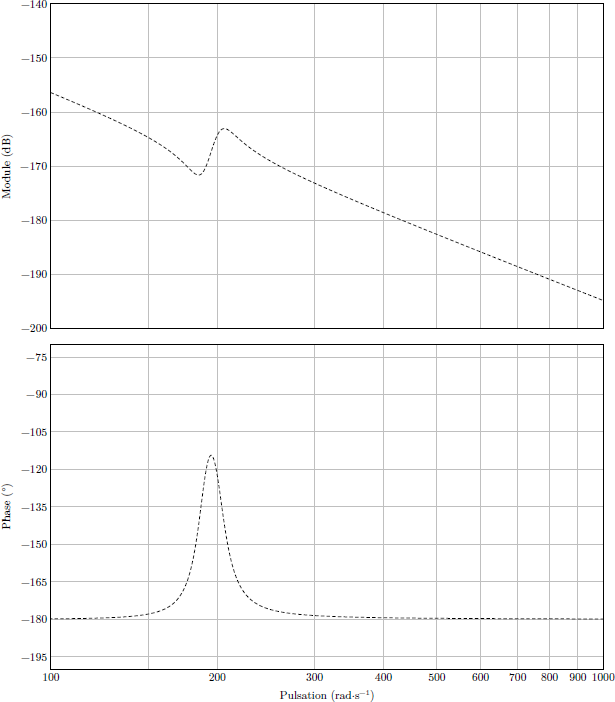
\includegraphics[width=\linewidth]{fig_dr}
%\caption{Modèle équivalent}
\end{marginfigure}
\fi
Le diagramme de Bode associé à la fonction de transfert $N_2(p)$ est représenté ci-contre.




\question{Compléter ce diagramme par les tracés asymptotiques en module et en phase, et conclure sur la
cohérence du diagramme donné.}
\ifprof
\begin{corrige}
D'après le diagramme asymptotique donné, on a nécessairement $\omega_1<\omega_2$. On peut dresser un tableau des variations à partir de la fonction de transfert $N_2(p)$. 
\begin{center}
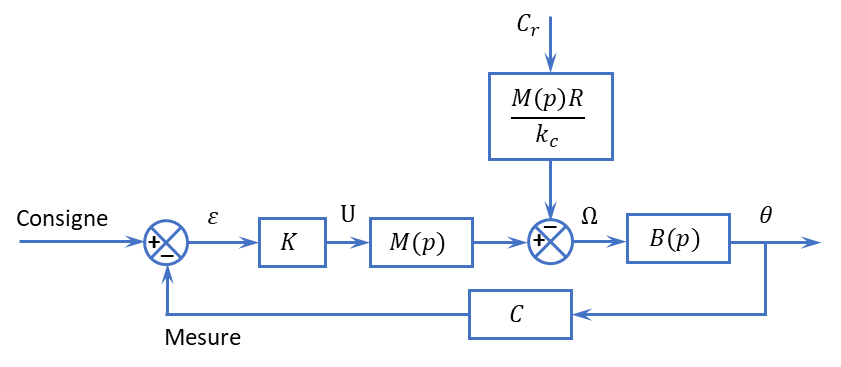
\includegraphics[width=.7\linewidth]{fig_06}

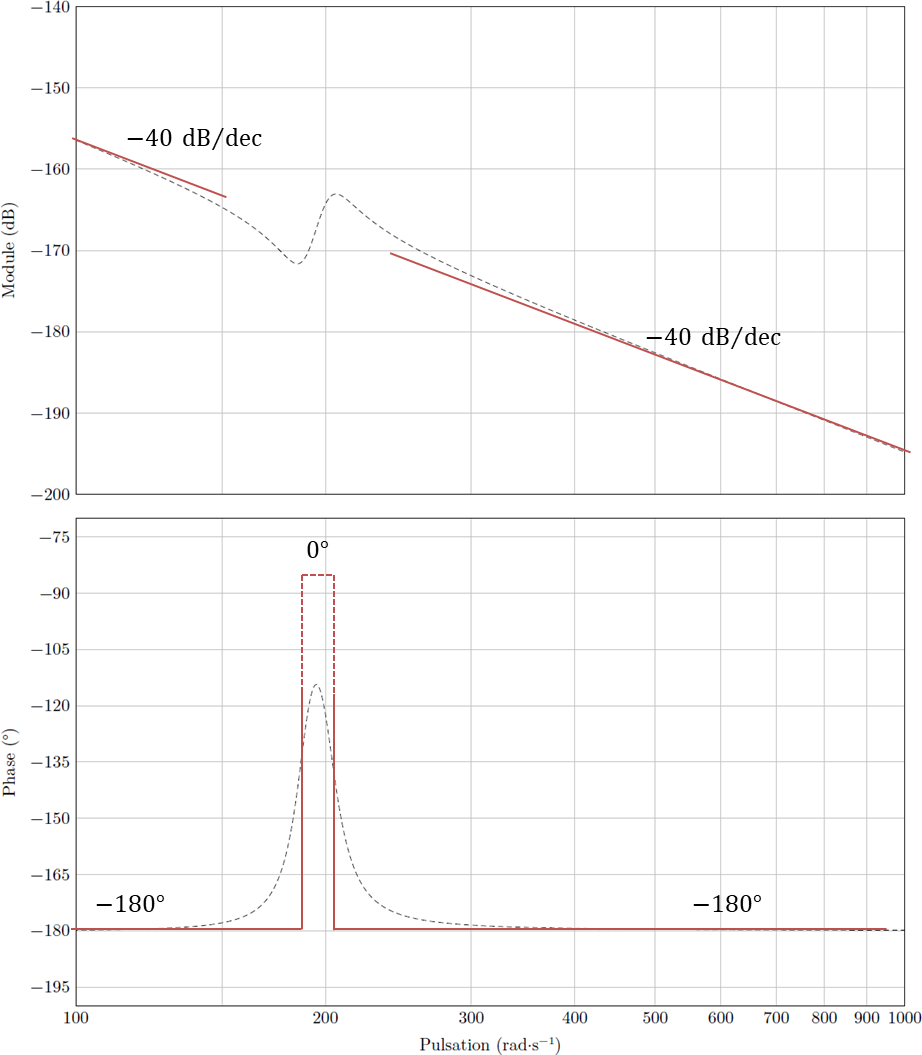
\includegraphics[width=.7\linewidth]{fig_07}
%\textit{}
\end{center}
\end{corrige}
\else
\fi

\question{Au regard des valeurs numériques, montrer que la fonction de transfert $N_2(p)$ peut être approchée
par la fonction $N_{2 \text{app}}(p)=\dfrac{A}{p^2}$. En utilisant une couleur différente, tracer le diagramme de Bode associé à la
fonction de transfert $N_{2 \text{app}}(p)$ sur le document réponse et conclure sur la validité de ce modèle approché.}
\ifprof
\begin{corrige}
Si le système n'est pas sollicité par des pulsations comprises entre 150 et \SI{250}{rad.s^{-1}}, on peut modéliser $N_2(p)$ par un double intégrateur. 
Le gain dB est donc  $20\log A - 20 \log \omega^2$.  Pour $\omega=\SI{500}{rad.s^{-1}}$ on a $20\log A - 20 \log 500^2=-182,5 \Rightarrow \log A = \dfrac{20 \log 500^2-182,5}{20}$ et $A=1,87\cdot 10^{-4}$.
\end{corrige}
\else
\fi

\ifprof
\else

\begin{marginfigure}
\centering
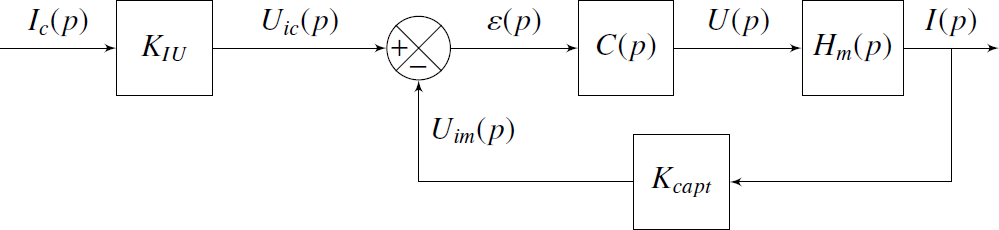
\includegraphics[width=\linewidth]{fig_13}
\caption{Modèle de synthèse de la régulation en position $z_1(t)$ du porte-outil \label{fig_13}}
\end{marginfigure}

Le modèle approché ($N_{2 \text{app}}(p)$) est retenu pour la suite de l’étude. Le schéma bloc modélisant la régulation de
la position $z_1(t)$ est donné en figure \autoref{fig_13}, en considérant un correcteur proportionnel de gain $K_p$.


\fi


\question{Justifier qu’une correction proportionnelle ne permet pas de respecter l’ensemble des critères du diagramme
des exigences de la \autoref{fig_08}.}
\ifprof
\begin{corrige}
Dans le cas, la FTBO est de classe 2.
\begin{itemize}
\item \textbf{req 1.1} : $M\varphi = 60\degres$ : impossible à respecter la phase sera toujours de $\SI{-180}{\degres}$.
\item \textbf{req 1.2} : $\omega_{\SI{0}{dB}}=\SI{200}{rad.s^{-1}}$ : critère non respecté (cf diagramme de Bode).
\item \textbf{req 1.4} : erreur en régime permanent : $\Delta c < \SI{40}{\mu m}$ pour un échelon d'amplitude $f_{c0}=\SI{1}{kN}$ : critère non respecté (pas d'intégrateur avant la perturbation).
\item \textbf{req 1.5} : défaut de la roue $\Delta u < \SI{30}{\mu m}$ lorsque la perturbation est sinusoïdale.
\end{itemize}

La correction proportionnelle ne permet donc pas de respecter tous les critères du cahier des charges.


\end{corrige}
\else
\fi

\subsection*{Analyse de l'influence d'un paramètre}

On a d'une part $Q(p) =Q_c (p)-Z_2(p)H_r (p)$. 

\marginnote{D’un point de vue numérique, $K_f = 1,5 \times 10^9 \si{N.m^{-2}}$ et $\tau = \SI{1}{s}$. }

D'autre part, la quantité de matière enlevée est donnée par $q(t)=q_c(t)-z_2(t)+z_2\left( t-\tau\right)$ où $\tau$ est la durée nécessaire à la roue pour effectuer
un tour complet. 



\question{Déterminer $H_r(p)$ en fonction de $\tau$.}
\ifprof
\begin{corrige}
D'après le schéma-blocs, $Q(p)=Q_c(p)-Z_2(p)H_r(p)$. 
D'après les équations données et en utilisant le théorème du retard, on a $Q(p)=Q_c(p)-Z_2(p)+Z_2(p)e^{-\tau p}=Q_c(p)-Z_2(p)\left(1-e^{-\tau p}\right)$. En conséquence, $H_r(p)=1-e^{-\tau p}$.
\end{corrige}
\else
\fi

Le schéma-blocs retenu est donné ci-contre. 

\ifprof
\else
\begin{marginfigure}
\centering
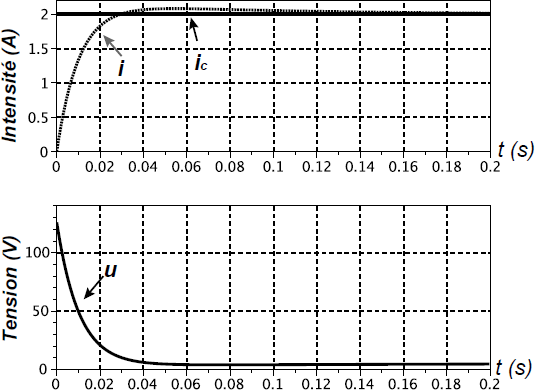
\includegraphics[width=\linewidth]{fig_16}
\caption{Modèle équivalent de la chaîne d'asservissement complète\label{fig_16}}
\end{marginfigure}


La \autoref{fig_17} représente le diagramme de Bode de la fonction de transfert en boucle ouverte du système modélisé
\autoref{fig_16}, avec $b=\dfrac{5\times 10^{-2}}{\pi} \si{mm.rad^{-1}}$

\begin{figure}[H]
\centering
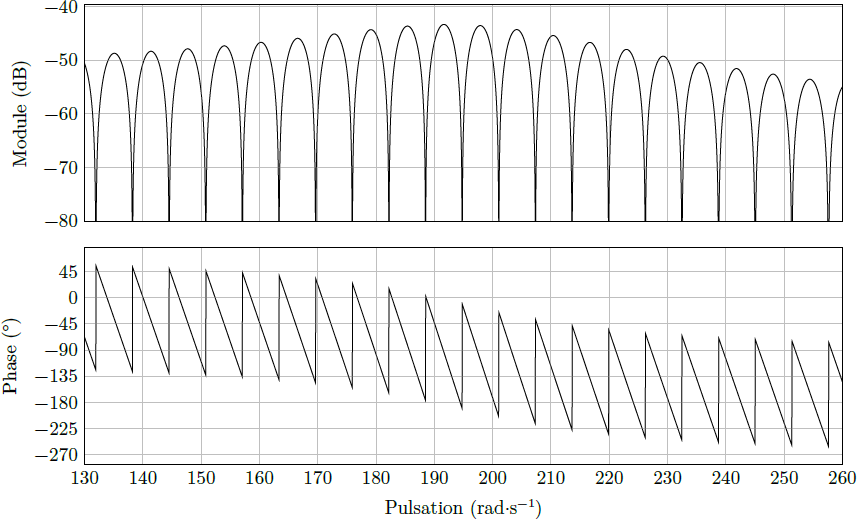
\includegraphics[width=\linewidth]{fig_17}
\caption{Diagramme de Bode de la boucle ouverte du schéma-blocs\label{fig_17}}
\end{figure}

Les « zéros de transmission » d’une fonction de transfert $H(p)$ correspondent aux pulsations $\omega$ pour lesquelles
$H\left(j \omega\right)$ est nul.

\fi

\question{Préciser l’expression de la fonction de transfert en boucle ouverte de la figure \autoref{fig_16} puis vérifier la cohérence du diagramme de Bode de la \autoref{fig_17}  en analysant les « zéros de transmission ».}
\ifprof
\begin{corrige}
$\text{FTBO}(p)=bK_f S(p)H_r(p)= \dfrac{bK_f}{K+\lambda p +m_2 p^2}\left(1-e^{-\tau p}\right) = H_2(p)\cdot H_r(p)$.

On a $G_{\text{dB}}(\omega)=G_{\text{dB2}}(\omega) + G_{\text{dBr}}(\omega)$.

$G_{\text{dBr}}(\omega) = 20\log \left|1-e^{-j\tau \omega} \right|=20\log 
\sqrt{\left( 1-\cos \left(-\tau \omega \right)\right)^2 + \left( \sin \left(-\tau \omega \right)\right)^2 } = 20\log \sqrt{2-2\cos \left( \tau \omega \right)}$.

On a donc :
\begin{itemize}
\item pour $\omega=\dfrac{k2\pi }{\tau}$ avec $k\in \mathbb{Z}^*$ et $G_{\text{dBr}}(\omega) \to -\infty $;
\item pour $\omega=\dfrac{\pi + k2\pi }{\tau}$ avec $k\in \mathbb{Z}^*$ et $G_{\text{dBr}}(\omega) = 20 \log 2$.
\end{itemize}

Le diagramme en gain montre alors l'addition d'un gain du second ordre et d'un gain périodique. Les << zéros de transmission >> correspondent aux pulsations $\omega=\dfrac{k2\pi }{\tau}$.

Pour la phase, $\varphi_{\text{BO}}\left( \omega\right)=\varphi_2\left( \omega\right)+\arg\left( 1-\cos\left( -\tau\omega\right) - j\sin\left(-\tau\omega\right)\right)$. Or $1-\cos\left( -\tau\omega\right) = 1-\cos\left( \tau \omega \right) \geq 0$. On a donc 
 $\varphi_{\text{BO}}=\varphi_2\left( \omega\right)+\arctan \left(\dfrac{\sin\left( \tau\omega\right)}{1-\cos\left( \tau\omega\right)} \right)$.

Le diagramme de  phase est la somme d'une phase d'un système du second ordre et d'un signal $\dfrac{2\pi}{\tau}$ périodique. 

\end{corrige}
\else
\fi

\question{Déterminer un ordre de grandeur du paramètre $b$ permettant de conserver la stabilité du système en
boucle fermée. Conclure sur la compatibilité de cette valeur maximale avec un bon amortissement de l’asservissement.}
\ifprof
\begin{corrige}
Pour garantir la stabilité en BF, il faut assurer un gain négatif en BO. D'après le diagramme de gain, le gain maximal relevé est de \SI{45}{dB}. Il faudrait donc ajouter un gain supplémentaire $b'$ tel que $20\log b' = 45$ soit $b'=10^{45/20}=177$. Au bilan, on aurait donc $b_{\text{lim}}=b' b = 177\times \dfrac{5\cdot 10^{-2}}{\pi}=
\SI{2,83}{mm.rad^{-1}}$.

Il faudrait déterminer si une augmentation de $b$ réduit l'amortissement de l'asservissement. 
\end{corrige}
\else
\fi

\ifprof
\else
\ifcolle
\else
\begin{solution}
\begin{enumerate}
\item $H_1(p)=\lambda p+K$, $H_2(p)=\dfrac{1}{m_1p^2  + \lambda p+K}$, $H_3(p)=\lambda p+K$,  $H_4(p)=\dfrac{1}{m_2p^2  + \lambda p+K}$.
\item $N_1(p)=H_1(p)H_4(p)$ et $N_2(p)=\dfrac{H_2(p)}{1-H_1(p)H_2(p) H_3(p)H_4(p)}$.
\item 	$\omega_1^2=\dfrac{K}{m_2}$, 
	$\omega_2^2=K\dfrac{m_1+m_2}{m_1m_2}$, 
	$\xi_1=\dfrac{\lambda}{2  \sqrt{m_2K}}$ et 
	$\xi_2=\lambda\dfrac{\sqrt{m_1+ m_2}}{2\sqrt{Km_1m_2}}$.
\item .
\item 	$A=1,87\cdot 10^{-4}$.
\item 	.
\item 	$H_r(p)=1-e^{-\tau p}$.
\item 	.
\item $b_{\text{lim}}=\SI{2,83}{mm.rad^{-1}}$.
\end{enumerate}
\end{solution}
\fi
\fi

\ifprof
\else
\begin{marginfigure}[-3cm]
\centering

\includegraphics[width=3cm]{Cy_01_Ch_02_Colle_03_qr}
\end{marginfigure}
\fi



